\section{Definition and Comparison to Stream Ciphers}

In symmetric cryptography, block ciphers and stream ciphers are two main types.

\paragraph{Stream ciphers} encrypt data one bit or one byte at a time. 
They use a \textit{keystream}, where each keystream bit is added to a plaintext bit individually.

\paragraph{Block ciphers} process fixed-size blocks of data, with each block encrypted separately.


\begin{figure}[h]
    \centering
    \begin{subfigure}[b]{0.45\textwidth}
        \centering
        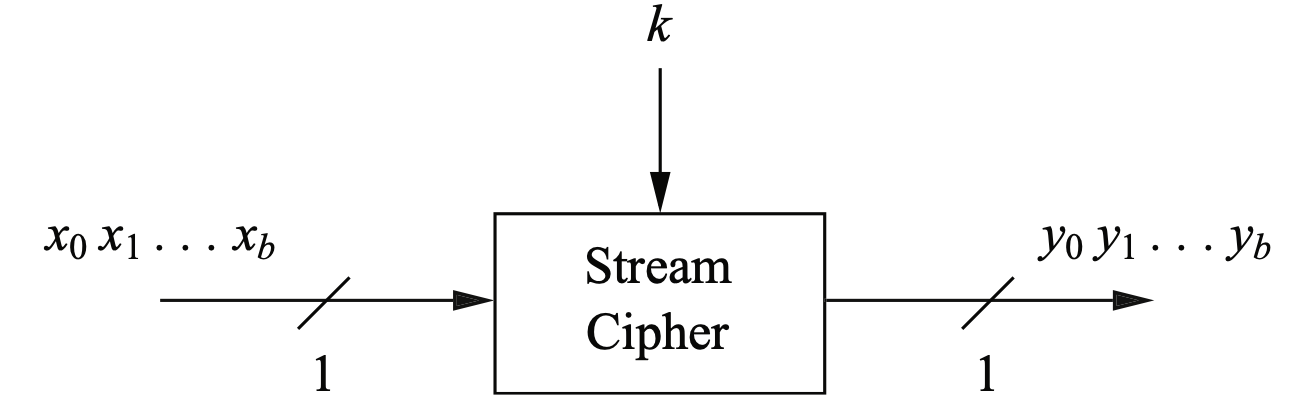
\includegraphics[width=\textwidth]{streamc.png}
        \caption{Stream cipher operation}
        \label{fig:stream_cipher}
    \end{subfigure}
    \hfill
    \begin{subfigure}[b]{0.45\textwidth}
        \centering
        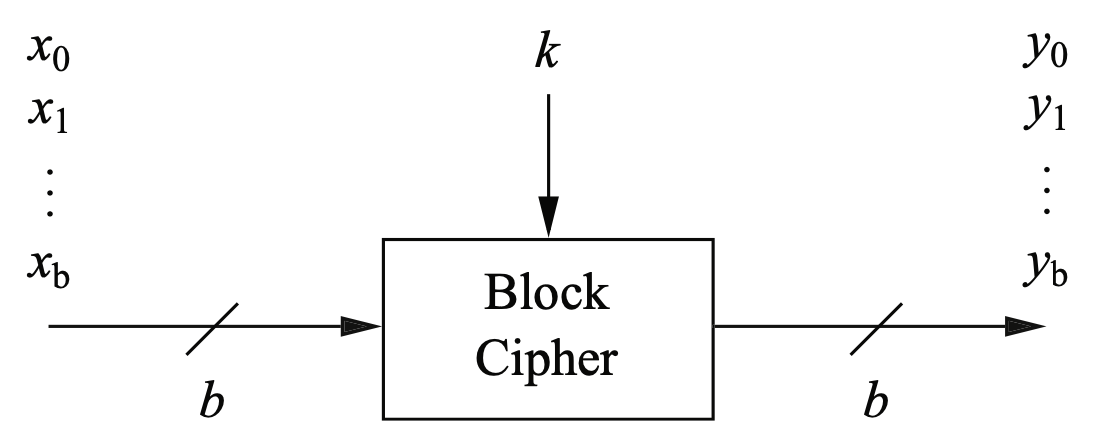
\includegraphics[width=.8\textwidth]{blockc.png}
        \caption{Block cipher operation}
        \label{fig:block_cipher}
    \end{subfigure}
    \caption{Comparison of stream and block cipher operations}
    \label{fig:cipher_comparison}
\end{figure}



\begin{table}[h]
\centering
\begin{tabular}{|c|c|}
\hline
\textbf{Block Cipher} & \textbf{Stream Cipher} \\
\hline
Encrypts chunks (blocks) & Encrypts continuously, bit by bit \\
\hline
Offers more security when used properly & Can be faster and have less delay \\
\hline
\end{tabular}
\caption{Comparison between block cipher and stream cipher.}
\label{tab:block_vs_stream}
\end{table}